%%%%%%%%%%%%%%%%%%%%%%%%%%%%%%%%%%%%%%%%%%%%%%%%%%%%%%%%%%%%%%%%%%%%%%%%%%%%%
%%%% Preamble
%%%%%%%%%%%%%%%%%%%%%%%%%%%%%%%%%%%%%%%%%%%%%%%%%%%%%%%%%%%%%%%%%%%%%%%%%%%%%

%%%% The uwthesis.sty file relies on the memoir class!
%%%% You should be using the memoir class anyway; it makes life easier:
%%%% http://www.ctan.org/tex-archive/macros/latex/contrib/memoir/
\def\bbbar{\ensuremath{\mathrm{b\bar{b}}}}

\documentclass[oneside, letterpaper, 12pt, oldfontcommands]{memoir}

%%%% Import uwthesis.sty to get official formatting, then set your variables.
\usepackage{uwthesis}
\usepackage{graphicx}
\usepackage{mathtools}

\settitle{Search for an MSSM Higgs Boson and Measurement of W+$b\bar{b}$, an Important Electroweak Background Process}
\setauthor{Isobel Rose Ojalvo}
\setdepartment{Physics}
\doctors % or \masters
\setgraddate{2013}
\setdefensedate{1 February 2013} % or whatever format you want

%%%% Members of the Final Oral Committee (FOC)
%%%% Give name, rank, and department
%%%% 
\setfoca{Wesley Smith}{Professor}{Physics} % <- Your advisor
\setfocb{Sridhara Dasu}{Professor}{Physics}

%%%% Your abstract, used for the UMI abstract and in your front matter
\setabstract{%
  An awesome study of important things is presented.  
  I further describe my project here, but I will not exceed 350 words, 
  for that is strictly forbidden for the abstract of this document.  
  If you're submitting online, you can even put symbols 
  in your abstract and title, but you'll have to find out the HTML 
  character codes for the various symbols.
}

%%%%%%%%%%%%%%%%%%%%%%%%%%%%%%%%%%%%%%%%%%%%%%%%%%%%%%%%%%%%%%%%%%%%%%%%%%%%%
%%%% Document
%%%%%%%%%%%%%%%%%%%%%%%%%%%%%%%%%%%%%%%%%%%%%%%%%%%%%%%%%%%%%%%%%%%%%%%%%%%%%

\begin{document}

% Tell the memoir class to set up lowercase roman for pagination, etc.
\frontmatter

%%%% Uncomment this to create a UMI abstract page.
%%%% If you are submitting electronically, however, this page is unnecessary.
% \theumiabstract

% The title page
\thetitlepage
\clearpage

% The copyright page, if you want to pay the fee and register copyright.
\thecopyrightpage
\cleardoublepage

% These above pages should not be counted, so we reset the counter to 1.
\setcounter{page}{1}

% An abstract may be required by your department.
\section{Abstract}
\uwabstract
\cleardoublepage

% Acknowledgements go here if you want to include them.
\section{Acknowledgements}
This is where any acknowledgements would go.
\clearpage

% Table of contents
\maxtocdepth{subsection}
\tableofcontents* % the * means that there isn't an entry for the TOC itself
% \clearpage
 \listoffigures*  % if you have any figures
% \clearpage
% \listoftables   % if you have any tables

% Tell the memoir class to set up normal pagination, etc. for the main doc
\mainmatter

\chapter{The Standard Model}
\section{A Historical Approach to High Energy Physics}
\section{Quarks, Leptons and Gauge Bosons}
\section{The Standard Model Higgs Boson}
\section{\bbbar Production at the LHC}

\chapter{Supersymmetry and MSSM}
\section{Minimally Supersymmetric Standard Model}
\section{MSSM Higgs Production}

\chapter{Experimental Setup}
\section{The Large Hadron Collider}
\section{Layout and Operation}
\section{Operating Conditions 2011 and 2012 Runs}

\chapter{The Compact Muon Solenoid Experiment}
 \section{Coordinate System}
The CMS detector is located on the LHC and is the experiment furtherest from the
CERN Meyrin site; its position on the LHC ring can be seen in figure \ref{fig:LHCRings}
The CMS coordinate system is oriented such that the x-axis points to the center of the LHC
ring. 
\begin{figure}[hb]
  \centering
	\includegraphics[width=0.75\textwidth]{images/LHCLayout.png}
  	\caption[e/$\gamma$ LHC Layout]
   	{LHC and Experiments Layout}
	\label{fig:LHCRings}
\end{figure}
The y-axis points vertically upward, perpendicular to the Earth's surface,
the z-axis is in the direction of the beam to the west. The angle $\phi$ is measured
azimuthally starting from the x-axis in the x-y plane, the radial coordinate in this plane
is denoted by r. The polar angle $\theta$ extends in the r-z plane and, importantly,
is used in the definition of pseudorapidity, $\eta$, as, 
\begin{displaymath}
\eta=-\ln{\tan\frac{\theta}{2}}.
\end{displaymath}
The spatial coordinate $\eta$ is preferred over the coordinate $\phi$ for 
defining the angle of a particle relative to the beam axis since
the particle production in minimum bias collisions is constant as a function of $\eta$.
The LHC is a hadron collider, therefore, the energy in the parton-parton interaction
that initiates interesting physics cannot be known. However, it is known that 
the momentum in the direction transverse to the z-axis is ~0. Therefore,
the interesting observables (energy and momentum) are defined as transverse
to the beam by measuring their x and y components and denoted as transverse
momentum, $p_{T}$, and transverse energy, $E_{T}$.%%%add in pt=sqrt(px^2+py^2)^1/2
%Reference: The CMS Collaboration, Detector performance and software, Physics
%Technical Design Report, Volume I (CMS TDR 8.1).
%\end{document}

 \section{Superconducting Magnet}%citations done
When designing a particle detector, choice of magnet configuration drives
much of the detector layout and design; large bending power is required to precisely 
measure the momentum of high-energy charged particles. This forced the CMS
collaboration to choose superconducting technology for the magnets.
The superconducting solenoid magnet used in CMS was designed to reach a 4-T field;
during the 2011 and 2012 runs it was operated at a central magnetic flux
density of 3.8-T to reduce the effects of aging on the coil \cite[PreciseMappings].
The purpose of this magnetic field is to allow precise measurement of the 
momentum of charged particles, across a wide range of energies, originating from LHC collisions. 

For a charged particle in a uniform magnetic field the  momentum of the charged particle is given by,
\begin{displaymath}
p=qBr
\end{displaymath}  
Where p is the momentum of the particle, q is its charge, B is the 
magnetic field strength and r is the radius of the particle's trajectory.
The transverse momentum resolution depends on the magnetic field and
solenoid radius as
\begin{displaymath}
\frac{dp}{p}\propto\frac{p}{BL^{2}}
\end{displaymath}
%Therefore, 
%is used for the measurement of track momenta in the tracker 
%and to predict track bendin
%by reconstructing the path of charged particle in the tracker
\begin{figure}[hb]
  \centering
	\includegraphics[width=0.75\textwidth]{ECALimages/magnet.png}
  	\caption[CMS Solenoid Magnet Layout]
   	{CMS Solenoid Magnet Layout}
	\label{fig:magnetLayout}
\end{figure}

The super conducting magnet consists of two main parts, the superconducting
solenoid and the return yoke.
Due to structural constraints, the solenoid itself is 6.3m in diameter and 12.5 m in length,
this is large enough to allow the tracker, electromagnetic calorimeter
and the hadronic calorimeter to be contained within the solenoid. This is
a desirable characteristic as it limits the number of radiation
lengths of material between the nominal collision point and these detectors. The solenoid
is composed of 4 layers of NbTi windings due to the large number of ampere-turns required.
 The windings and support structure of the solenoid
are detailed in Figure \ref{fig:magnetLayout}. 
The magnetic field is given by,
\begin{displaymath}
B=\mu_{0}nI
\end{displaymath}
where $\mu_{0}$ is the magnetic constant, n is the number of turns per unit length and 
I is the current. 
The flux is returned by a 10,000 ton iron yoke which is composed of 11 elements, 6 endcap disks 
and 5 barrel wheels. The yoke also was designed to contain four muon stations. 
Both the solenoid cryostat system and the yoke also serve a dual purpose as a structural support 
for the CMS experiment. 
 %%%%%ADD IN TRACKER RESOLUTION
\section{Tracking System}
The tracker is CMS's inner-most detector. The purpose of the 
tracker is to reconstruct the trajectories of charged particles 
coming from the LHC collisions and measure the charged particle momenta. 
These charged particles leave a path in the tracker material referred to as a 'track'. %fix
These tracks are then used in the reconstruction of electrons, muons, taus, hadrons and jets 
and are also used to determine the primary vertex of an interaction. Additionally, 
the tracker can be used in the identification of displaced vertices which are located
away from the primary vertex; a displaced vertex (or 'secondary vertex') is 
a decay signature that is often present 
in heavy (b or c -flavored) jets.
As can be seen in Figure \ref{fig:trackerLayout}, the CMS tracker consists of two main 
detectors: an inner silicon pixel detector and an outer silicon strip detector. 
\begin{figure}[hb]
  \centering
	\includegraphics[width=1\textwidth]{trackerImages/trackerLayout.png}
  	\caption[CMS Tracker Layout]
   	{CMS Tracker layout}
	\label{fig:trackerLayout}
\end{figure}
Efficient reconstruction of collisions require a low hit occupancy, a high hit redundancy and a
fast response such that tracks can be identified reliably and attributed to the correct bunch crossing.
Low hit occupancy can be achieved with high granularity while high hit redundancy requires
many detector layers. These former two requirements are only achieved with a 
high power density of on detector electronics which require efficient cooling. 
Unfortunately, this directly conflicts with the goal to limit the material 
budget of the tracker; interaction with material results in Coulomb scattering,
bremsstrahlung, nuclear interactions and photon conversion. Finally, an extremely
high particle flux results in radiation damage to the silicon sensors mainly 
in the form of modifications to the silicon crystal lattice. 
The aforementioned objectives and constraints resulted in a tracker design 
based entirely on silicon detector technology. 
At 5.4 m in length and 2.2 m in diameter, the CMS tracker is the largest inner
silicon detector ever built in a high energy physics experiment.
\begin{figure}[hb]
  \centering
  \begin{subfigure}[b]{.45\textwidth}
	\includegraphics[width=\textwidth]{images/Tracker_Materials_x_vs_eta.eps} 
	\end{subfigure}	
   \begin{subfigure}[b]{.45\textwidth}
	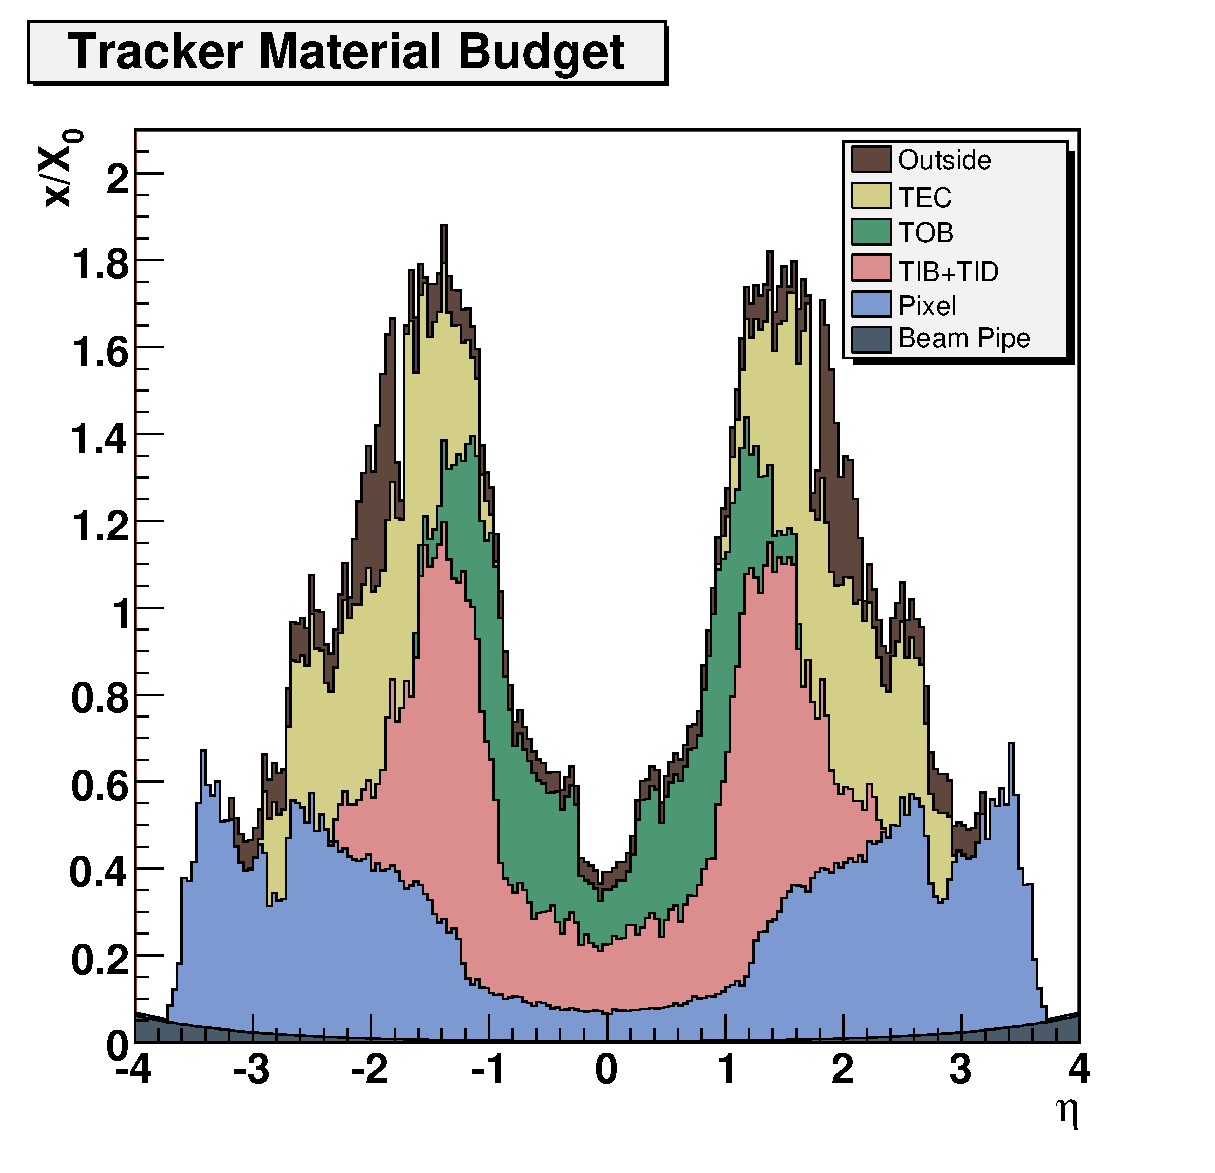
\includegraphics[width=\textwidth]{images/Tracker_SubDetectors_x_vs_eta.eps}
    \end{subfigure}	
  	\caption[Tracker Material Budget]
   	{Tracker material budget, x/$X_{0}$ vs. $\eta$}
	\label{fig:trackerMaterial}
\end{figure}

The material budget of the tracker can be characterized by the rate at which a particle
passing through it loses energy. The radiation length, $X_{0}$, is the 
mean distance over which a high-energy electron loses all but 1/$e$ 
of its energy by bremsstrahlung %citation needed p.291 PDG ------
and $\frac{7}{9}$ of the mean free path for pair production by 
a high-energy photon. Figure \ref{fig:trackerMaterial}
shows the material budget of the CMS tracker in terms of radiation length as a function of $\eta$. 
Due to the location of cabling, electronics and other services, the material budget of the 
tracker is at a minimum of 0.4 $X_{0}$ at $\eta \approx 0$ and increases to approximately 1.8 $X_{0}$
at $|\eta| \approx 1.4$, after which it decreases. 

%Resolution on the order of 10 micro meters http://arxiv.org/pdf/1007.1988.pdf
\subsection{Pixel Detector}%%%check to be sure where you say pixel system vs. pixel detector 
The pixel detector is the inner most detector of the tracking system and,
covering the region from 4 to 15 cm in radius, is the closest detector to 
the interaction point. It has a high granularity and contributes precise 
tracking points in $r-\phi$ and $z$ and is therefore responsible for a small impact 
parameter resolution that is important for b and c-jet secondary
vertex reconstruction and $\tau$-lepton secondary vertex reconstruction.

\begin{figure}[hb]
  \centering
	\includegraphics[width=0.7\textwidth]{images/pixelLayout.png}
  	\caption[Pixel System Layout]
   	{Pixel System Layout}
	\label{fig:pixelLayout}
\end{figure}

The pixel detector is made up of individual pixel cells with a size of 
100 $\times$ 150 $\mu m^{2}$; it has 66 million active elements and covers
a surface area of 1 $m^{2}$. The pixel detector is composed of three barrel 
layers and two endcap disks for which the pseudorapidity range from $-2.5<\eta<2.5$.
The three barrel layers are located at mean radii of 4.3, 7.3, and 10.2 cm. 
The endcap disks extend from 4.8 to 14.4 cm in radii are located at a mean distance
of $z=\pm35.5$ cm and $z=\pm48.5$ cm from the interaction point. 
As can be seen in figure \ref{fig:pixelLayout} this arrangement allows for 3 tracking points over 
almost the full $\eta$-range of the pixel system. Due to 
particles entering the detector at an average angle of $20^{\circ}$ 
charge-sharing between pixels is achieved which improves position resolution.

The pixel system has a zero-suppressed read out scheme with analog pulse
height read-out. This improves the position resolution due to charge sharing,
it helps to separate signal and noise hits as well as to identify large hit 
clusters from overlapping tracks.
A position resolution on the order of 10 $\mu m$ is achieved.

\subsection{Silicon Strip Tracker}
The silicon strip detector is located outside the inner pixel detector, 
It extends from 25 cm to 110 cm in radius and pseudorapidity up to $|\eta|<2.5$. 
This region has a particle flux on 
the order of 100 times less than what is seen by the inner most layers of 
the pixel detector. It is a complementary system to the inner pixel
detector and has a lower granularity. The silicon strip detector 
has 9.3 million active elements over a total surface area of 198 m$^{2}$
and consists of 3 large subsystems. As can be seen in figure \ref{fig:trackerLayout}, 
the Tracker Inner Barrel and Disks (TIB/TID) extend in radius to
55cm and are composed of four barrel layers with three disks at each.
The Tracker Outer Barrel (TOB) consists of six barrel layers and extends to $\pm118$ cm
in z. Extending beyond this in the z-direction, the Tracker EndCaps (TEC+ and TEX- where the plus and minus
indicate the direction in z) are located from 124cm $<|z|<$280 cm. They are composed of 
nine disks which are populated with up to seven rings of radial-strip silicon detectors.
The combined layouts of the pixel detector and silicon strip detector
result in 8 to 14 high precision measurements of track impact points for 
$|\eta|<2.4$.
  \section{Electromagnetic Calorimeter}
Directly outside of the tracking system lies the electromagnetic calorimeter 
(ECAL) of CMS. The driving criteria of the ECAL design is to provide capability
to detect and measure the decay to two photons of the Higgs Boson. The 
ECAL is designed with the objective of a
fast response time, a fine granularity and resistance to the effects of radiation.
Therefore, recently advanced lead tungstate (PbWO$_{4}$) technology was chosen. 
A preshower detector is placed in front of the endcap. Avalanche photodiodes (APDs)
are used as photodetectors in the barrel and vacuum phototriodes (VPTs) in the
endcaps.
The layout of the CMS ECAL is shown in Figure %Include ECAL figure
The barrel part of the ECAL (EB) covers the pseudorapidity range $|\eta|<1.479$
the endcap part covers the rapidity range $1.479<|\eta|<3.0$.
\subsection{Lead Tungstate Crystals}
The ECAL is composed of 75,848 PbWO$_{4}$ crystals: 61,200 mounted in the 
central barrel part, closed by 7,324 crystals in each of the two endcaps. They 
have a high density of 8.28$g/cm^{3}$ and a short radiation length of 0.89cm. 
The Moli$\grave{e}$re radius (radius of a cylinder containing 90\% of the shower's energy deposit) 
is only 2.2cm. These characteristics result in a fine granularity and a compact
calorimeter. Futhermore, the scintillation decay time of these crystals is of the
same order of magnitude as the LHC bunch crossing time whereby 80\% of 
the light is emitted in 25ns. 
\subsection{Energy Resolution}
The energy resolution in the ECAL can be parameterized as in the following equation:
\begin{displaymath}
\left\frac{\sigma}{E}\right^{2}=\left\frac{S}{\sqrt{E}})^{2}\right+\left\frac{N}{E}^{2}\right+C^{2}
\end{displaymath}
where $S$ is the stochastic term, $N$ the noise term, and $C$ the constant term. 
The individual contributions are described in the following paragraphs.


 \section{Hadronic Calorimeter}
The CMS detector is designed to study a wide range of high energy 
physics processes; measurement of hadronic jets and neutrinos or
physics processes which result in missing transverse energy require
a hadronic calorimeter. 
Located outside the Electromagnetic Calorimeter but still within the
superconducting magnet volume is stationed the Hadronic Calorimeter (HCAL).
The Hadronic Calorimeter is a sampling calorimeter: it consists of layered 
sheets of scintillators interleaved with brass absorber plates. Figure %reference figure for HCAL
shows the placement of the of the four regions of the HCAL, the HCAL Barrel (HB),
the HCAL Endcap (HE), the HCAL Forward (HF) and the outer HCAL (HO). 
%The last of these, the outter HCAL, was not active for the 2011/2012 runs. 
The barrel and endcap HCALs, HB and HE, are located within the 
solenoid magnet. The HB extends across $|\eta|<1.3$ and the HE extends from ___


Due to the technical and environmental demands the HF is based on
Cherenkov Radiationg Quartz technology. The forward region has an overall 
higher particle flux and 



 \section{Muon System}
  \subsection{Drift Tube Chambers}
  \subsection{Cathode Strip Chambers}
  \subsection{Resistive Plate Chambers}
 \section{Trigger}
  \subsection{Level 1 Trigger}
 \section{Regional Calorimeter Trigger}
 \section{High Level Trigger}
\chapter{Event Reconstruction}
\section{Tracks and Vertices}
\section{Electron Reconstruction and ID}
\section{Muon Reconstruction and ID}
\section{Tau Reconstruction and ID}
\section{Jet Reconstruction}
\subsection{Identification of Jets Originating from b-Quarks}
\section{Missing Transverse Energy}
\chapter{Event Simulation}

\chapter{Measurement of W plus \bbbar Pair Production}
\section{Initial Event Selection}
\section{Irreducible Backgrounds}
\section{Systematic Uncertainty}
\section{Signal Extraction}
\section{Results}

\chapter{Search for MSSM Higgs Boson}
\section{Initial Event Selection}
\section{Background Modeling}
\section{Systematic Uncertainty}
\section{Exclusion}
\section{Results}


\chapter{Conclusions}
\section{Future Outlook}

\end{document}



The Standard Model
-Background
-Quarks, Leptons, Gauge Bosons
-Standard Model Higgs
-bbbar production at the LHC

Supersymmetry and MSSM
-The Minimal Supersymmetric Standard Model
-MSSM Higgs production

Experimental Setup
- The LHC
- Layout and Operation
- Operating Conditions 2011/2012 runs

The Compact Muon Solenoid Experiment
-Coordinate System
-Magnet
-Tracking System
  --Pixel Detector
  --Silicon Strip Tracker
-Electromagnetic Calorimeter
-Hadronic Calorimeter
-Muon System
  --Drift Tube Chambers
  --Cathode Strip Chambers
  --Resistive Plate Chambers
-Trigger
-- L1 Trigger
--Regional Calorimeter Trigger
--High Level Trigger

Event Reconstruction
-Tracks and Vertices
-Electron Reconstruction and ID
-Muon Reconstruction and ID
-Tau Reconstruction and ID
-Jet Reconstruction
  -- Identification of Jets originating from b quarks
-Missing Transverse Energy

Measurement of W boson plus bbbar pair Production
-Systematics
-Backgrounds
-Signal Extraction
-Result

Search for MSSM Higgs Boson
-Systematics
-Backgrounds
-Limit
-Result

Conclusions
